%=========================================================
% Peripheral : I2C
%=========================================================
\section{Peripheral : I2C}

\begin{description}

    \item[Overview]\mbox{}\\
        This module is a simple master I2C interface based on OpenCores I2C Master controller (http://www.opencores.org/projects/i2c/) by Richard Herveille. Please refer to the IP’s document for more details. The I2C can generate interrupt requests when (A) a byte transfer has been completed or (B) arbitration is lost.

    \item[Input / Output Signals]\mbox{}\\
        Input / Output signals of UART are shown in Table \ref{tb:IOSIGNALS_I2C}. The I/O buffers for SCL and SDA should be prepared in upper layer as shown in Figure \ref{fig:I2C_BUFFER}.

%-------------------------------
\begin{table}[H]
    \begin{adjustbox}{scale={0.65}{0.8}}
    \textsf{
    \begin{tabular}{|L{4cm}{2cm}{t}|L{4cm}{2cm}{t}|L{2cm}{1cm}{t}|L{7cm}{6cm}{t}|L{10cm}{6cm}{t}|L{3cm}{2cm}{t}|}
        \hline
        %-------------------------------------
        \rowcolor{LightPurple}
        \textbf{Group} &
        \textbf{Direction} &
        \textbf{Width} &
        \textbf{Name} &
        \textbf{Description} &
        \textbf{Note}
        \nextRow \hline
        %-------------------------------------
        System & input  & ~ & RES & Reset & ~
        \nextRow \hline
        %-------------------------------------
        System & input  & ~ & CLK & System Clock & ~
        \nextRow \hline
        %-------------------------------------
        AHB    & input  & ~                   & S\_HSEL      & AHB Lite Slave Select & ignored
        \nextRow \hline
        %-------------------------------------
        AHB    & input  & \lbrack  1:0\rbrack & S\_HTRANS    & AHB Lite Slave Transfer Type & ~
        \nextRow \hline
        %-------------------------------------
        AHB    & input  & ~                   & S\_HWRITE    & AHB Lite Slave Write & ~
        \nextRow \hline
        %-------------------------------------
        AHB    & input  &                     & S\_HMASTLOCK & AHB Lite Slave Locked Transfer & ignored
        \nextRow \hline
        %-------------------------------------
        AHB    & input  & \lbrack  2:0\rbrack & S\_HSIZE     & AHB Lite Slave Access Size & ~
        \nextRow \hline
        %-------------------------------------
        AHB    & input  & \lbrack  2:0\rbrack & S\_HBURST    & AHB Lite Slave Burst Access & ignored
        \nextRow \hline
        %-------------------------------------
        AHB    & input  & \lbrack  3:0\rbrack & S\_HPROT     & AHB Lite Slave Protection & ignored
        \nextRow \hline
        %-------------------------------------
        AHB    & input  & \lbrack 31:0\rbrack & S\_HADDR     & AHB Lite Slave Address & ~
        \nextRow \hline
        %-------------------------------------
        AHB    & input  & \lbrack 31:0\rbrack & S\_HWDATA    & AHB Lite Slave Write Data & ~
        \nextRow \hline
        %-------------------------------------
        AHB    & input  & ~                   & S\_HREADY    & AHB Lite Slave Ready Input & ~
        \nextRow \hline
        %-------------------------------------
        AHB    & output & ~                   & S\_HREADYOUT & AHB Lite Slave Ready Output & ~
        \nextRow \hline
        %-------------------------------------
        AHB    & output & \lbrack 31:0\rbrack & S\_HRDATA    & AHB Lite Slave Read Data & ~
        \nextRow \hline
        %-------------------------------------
        AHB    & output & ~                   & S\_HRESP     & AHB Lite Slave Response & always output 0
        \nextRow \hline
        %-------------------------------------
        I2C    & input  & ~                   & I2C\_SCL\_I   & I2C SCL Input & ~
        \nextRow \hline
        %-------------------------------------
        I2C    & output & ~                   & I2C\_SCL\_O   & I2C SCL Output & ~
        \nextRow \hline
        %-------------------------------------
        I2C    & output & ~                   & I2C\_SCL\_OEN & I2C SCL Output Enable & ~
        \nextRow \hline
        %-------------------------------------
        I2C    & input  & ~                   & I2C\_SDA\_I   & I2C SDA Input & ~
        \nextRow \hline
        %-------------------------------------
        I2C    & output & ~                   & I2C\_SDA\_O   & I2C SDA Output & ~
        \nextRow \hline
        %-------------------------------------
        I2C    & output & ~                   & I2C\_SDA\_OEN & I2C SDA Output Enable & ~
        \nextRow \hline
        %-------------------------------------
        INT    & output & ~                   & IRQ\_I2C      & Interrupt Request & ~
        \nextRow \hline
        %-------------------------------------
    \end{tabular}
    }
    \end{adjustbox}
    \caption{Input / Output Signals of I2C}
    \label{tb:IOSIGNALS_I2C}
\end{table}
%-------------------------------
%-------------------------------
\begin{figure}[H]
    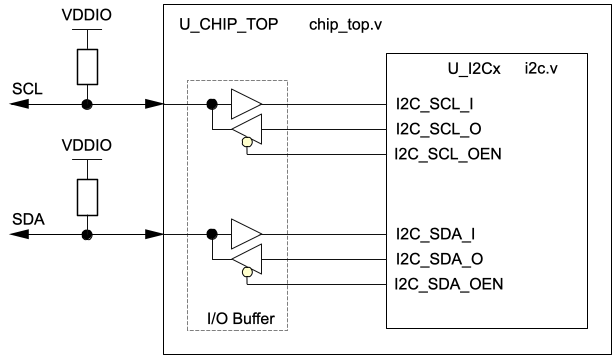
\includegraphics[width=0.8\columnwidth]{./Figure/I2C_BUFFER.png}
    \caption{I/O Buffers for I2C}
    \label{fig:I2C_BUFFER}
\end{figure}
%-------------------------------

    \item[Control Registers]\mbox{}\\
        Controls registers of I2C are shown in Table \ref{tb:REG_I2C_PRERL} to Table \ref{tb:REG_I2C_SR}. Please refer the technical document of the OpenCores I2C Master controller (http://www.opencores.org/projects/i2c/).
 
\end{description}

%-------------------------------
\begin{table}[H]
    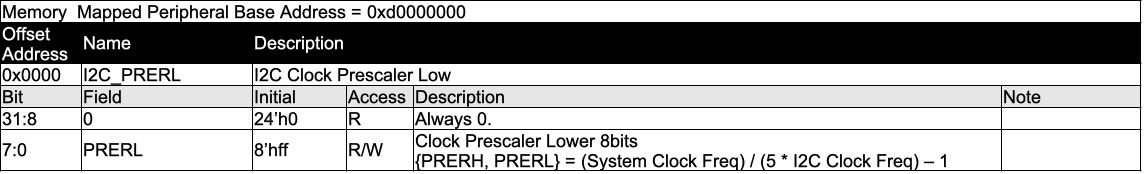
\includegraphics[width=1.0\columnwidth]{./Table/REG_I2C_PRERL.png}
    \caption{I2C\_PRERL}
    \label{tb:REG_I2C_PRERL}
\end{table}
%-------------------------------
%-------------------------------
\begin{table}[H]
    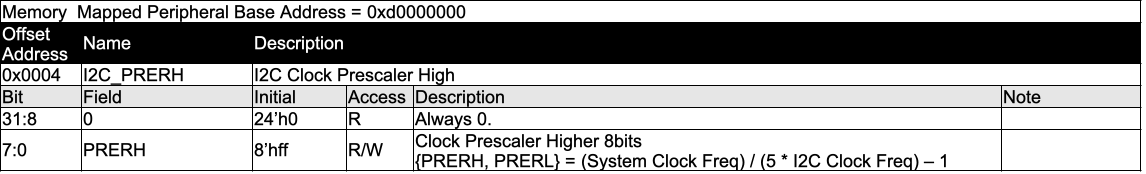
\includegraphics[width=1.0\columnwidth]{./Table/REG_I2C_PRERH.png}
    \caption{I2C\_PRERH}
    \label{tb:REG_I2C_PRERH}
\end{table}
%-------------------------------
%-------------------------------
\begin{table}[H]
    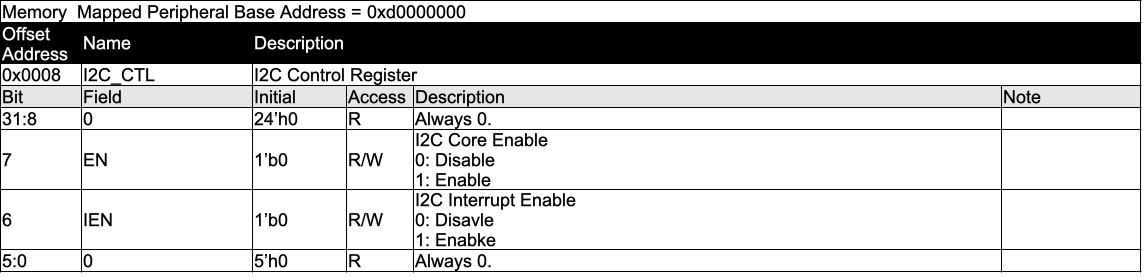
\includegraphics[width=1.0\columnwidth]{./Table/REG_I2C_CTL.png}
    \caption{I2C\_CTL}
    \label{tb:REG_I2C_CTL}
\end{table}
%-------------------------------
%-------------------------------
\begin{table}[H]
    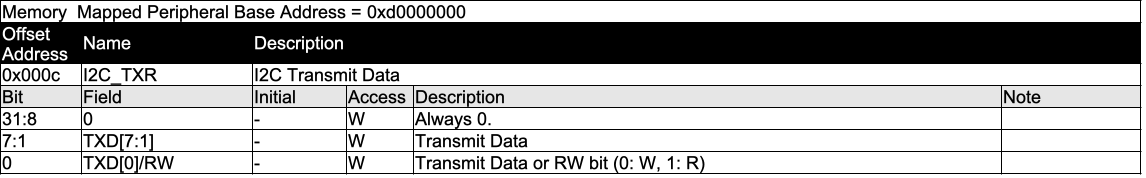
\includegraphics[width=1.0\columnwidth]{./Table/REG_I2C_TXR.png}
    \caption{I2C\_TXR}
    \label{tb:REG_I2C_TXR}
\end{table}
%-------------------------------
%-------------------------------
\begin{table}[H]
    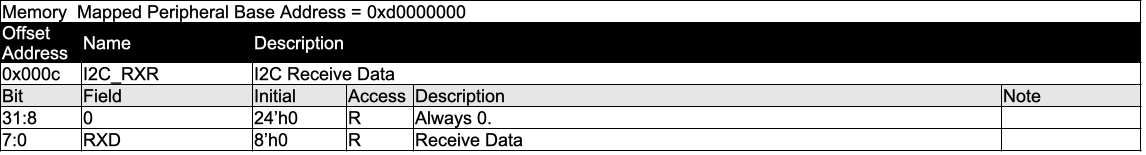
\includegraphics[width=1.0\columnwidth]{./Table/REG_I2C_RXR.png}
    \caption{I2C\_RXR}
    \label{tb:REG_I2C_RXR}
\end{table}
%-------------------------------
%-------------------------------
\begin{table}[H]
    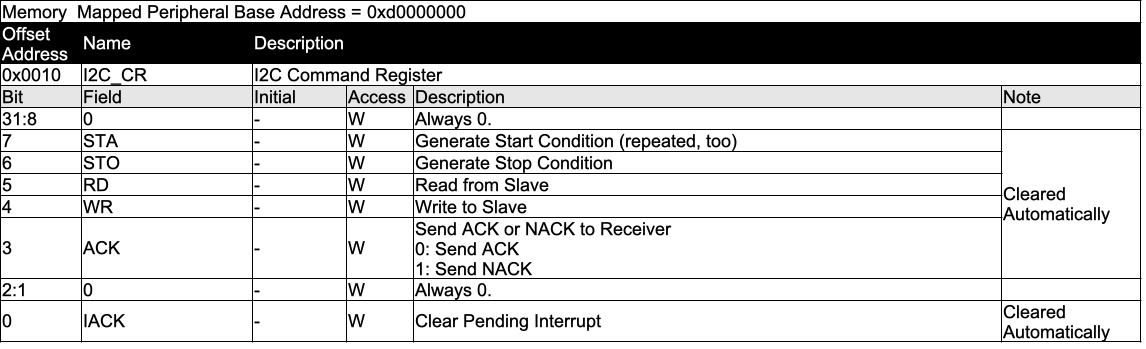
\includegraphics[width=1.0\columnwidth]{./Table/REG_I2C_CR.png}
    \caption{I2C\_CR}
    \label{tb:REG_I2C_CR}
\end{table}
%-------------------------------
%-------------------------------
\begin{table}[H]
    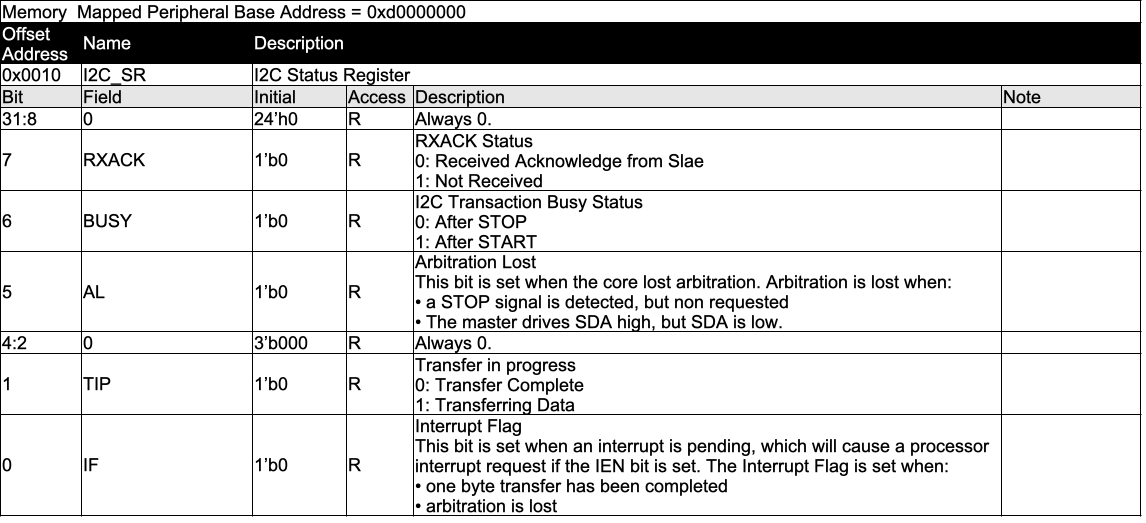
\includegraphics[width=1.0\columnwidth]{./Table/REG_I2C_SR.png}
    \caption{I2C\_SR}
    \label{tb:REG_I2C_SR}
\end{table}
%-------------------------------


